\documentclass{standalone}
\usepackage[T1]{fontenc}
\usepackage[utf8]{inputenc}
\usepackage{pgf,tikz}
\usepackage{setspace}
\usepackage{pgfplots}
\pgfplotsset{compat=1.12}

\begin{document}

\begin{tikzpicture}[scale=1]
       \begin{scope}[scale=1.0, xshift = -3cm, yshift=3cm, rotate=-20, ]
	 \node[rotate=-20] (module) {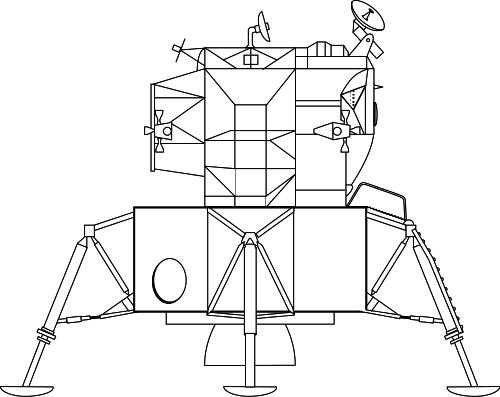
\includegraphics[width=4cm]{../../figures/apollo-moonlander.png}};
	 \draw[ultra thick, red, ->] (-1,0.3) arc (260:100:0.3) node[left, pos=0.5] (annot) {$u$};
	 \node[coordinate, pin=180:{attitude thrusters}] at (-0.8, 0.4) {};
	 \node[coordinate, pin=180:{main thruster}] at (-0.1, -1.2) {};
	 \draw[ultra thick, red, ->] (1.1,1) arc (80:-80:0.3);
	 \draw[ultra thick, red, ->] (0,-1.5) -- (0,-3);
	 \draw[ dashed, rotate=20] (0,0) -- (0,2.5);
	 \draw[ dashed, ] (0,0) -- (0,2.5);
	 \draw[->, rotate=20] (0,2) arc (90:70:2) node[above, pos=0.5] {$\theta$};
       \end{scope}
       \draw[->] (-6, 0) -- (6,0) node[below] {$z$};
     \begin{scope}[yshift=-1.8cm, xshift=-7cm, node distance=28mm, block/.style={rectangle, draw, minimum width=15mm}, sumnode/.style={circle, draw, inner sep=2pt}]
	 \node[coordinate] (input) {};
	 \node[block, right of=input,] (int1)  {$\frac{k_1}{s}$};
	 \node[block, right of=int1, ] (int2)  {$\frac{1}{s}$};
	 \node[block, right of=int2, ] (gain)  {$k_2$};
	 \node[block, right of=gain, ] (int3)  {$\frac{1}{s}$};
	 \node[coordinate, right of=int3] (output) {};

	 \draw[->] (input) -- node[above, pos=0.3] {$u(t)$} (int1);
	 \draw[->] (int1) -- node[above] {$\dot{\theta}(t)$} (int2);
	 \draw[->] (int2) -- node[above] {$\theta(t)$} (gain);
	 \draw[->] (gain) -- node[above] {$\ddot{z}(t)$} (int3);
	 \draw[->] (int3) -- node[above, near end] {$\dot{z}(t)$} (output);
       \end{scope}
     \end{tikzpicture}
   \end{document}
   